\subsection{Delays}

Delays are one of the most crucial parts of this project since most of the system is time-sensitive, meaning that there are specific time intervals that nearly all programs have to take into account to function properly. Both monostable and astable timers can be implemented using clock cycle counters in VHDL, but for this project, we have decided to use the well-know 555 timer so as to reduce the amount of GALs. We can define 2 different 555 timer configurations in our project:
%%maybe put pic of outside subsystem?
\begin{itemize}
    \item Delayed steady ON after a PGT
    \item Delayed impulse after a PGT
\end{itemize}

None of the two configurations are standard, meaning that they can't simply be referred to as a barebones monostable or astable configuration. We have used non-linear elements such as diodes to achieve the desired results. We will now go over them so as to explain how they work and what their purpose is:

\subsubsection{Delayed steady ON after a PGT}
\label{sec:DELAYED_STEADY}

As the name suggests, this first configuration turns the output Q (Pin 3) to a high state one second after a PGT occurs in the input. In this case, the input is connected to the 555's $V_{cc}$ pin. The circuit's diagram is as follows:

\begin{figure}[H]
    \centering
    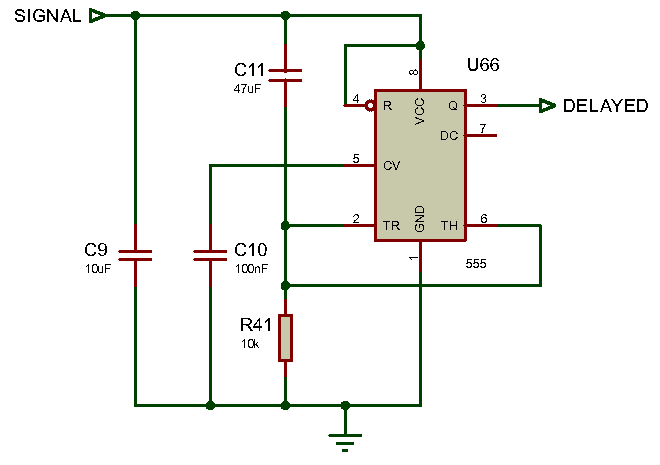
\includegraphics[scale = 1]{Graphics/DELAY/DELAY_STEADY.PDF}
    \caption{Delayed steady ON after a PGT}
    \label{fig:DELAY_STEADY}
\end{figure}

How this circuit works is through the RC network. The combination of the resistor and capacitor forms the RC network. This network determines the length of time it takes to charge the capacitor, i.e. the bigger the resistor and capacitor value, the longer the delay.\medskip

The reason why the circuit doesn't turn on automatically is because pin 2, the trigger pin, initially when the power turns on, is HIGH. This is because the capacitor hasn't charged up yet. Until the capacitor charges up, this pin is HIGH. Since the trigger pin is active LOW, the output will be off until this pin goes LOW. As the capacitor charges up and gets near the supply voltage it is connected to, the voltage at pin 2 decreases. When the voltage at pin 2 gets below 1/3 of the supply voltage, the pin is now LOW. When it is LOW, this is when the output goes HIGH, effectively delaying the input signal.\medskip

In this circuit, capacitors C9 and C10 are there just to decouple the input signal. They have nothing to do with the timing circuit. \medskip

This subassembly is used only once in our circuit. Its function is to delay the \emph{DONE} signal. The purpose of this is to give the Individual Digit Checking GALs some time to perform their operations before checking if the whole password is correct. This delay is needed to overcome the internal propagation delays of the GALs.\medskip


\subsubsection{Delayed impulse after a PGT}
\label{sec:DELAYED_PULSE}

This second circuit is very similar to the first one, the only difference being that instead of a steady ON after a PGT, it only outputs a short pulse after a delay. To achieve this behaviour two 555s have been connected to one another. The first one is connected in the same configuration that we described earlier, that is, it outputs a delayed steady ON after a PGT. The second 555 circuit is a bit more complex. In essence, it behaves as a monostable, as it only outputs a single pulse when triggered. The only difference is that to trigger a monostable, a NGT pulse has to be applied to the Trigger pin (Pin 2), but this cannot be achieved using out configuration as the output of the first 555 is a steady ON. \medskip

\clearpage

To get around this problem, we have used a special tipe of monostable which operation we will describe below.\medskip

\begin{figure}[H]
    \centering
    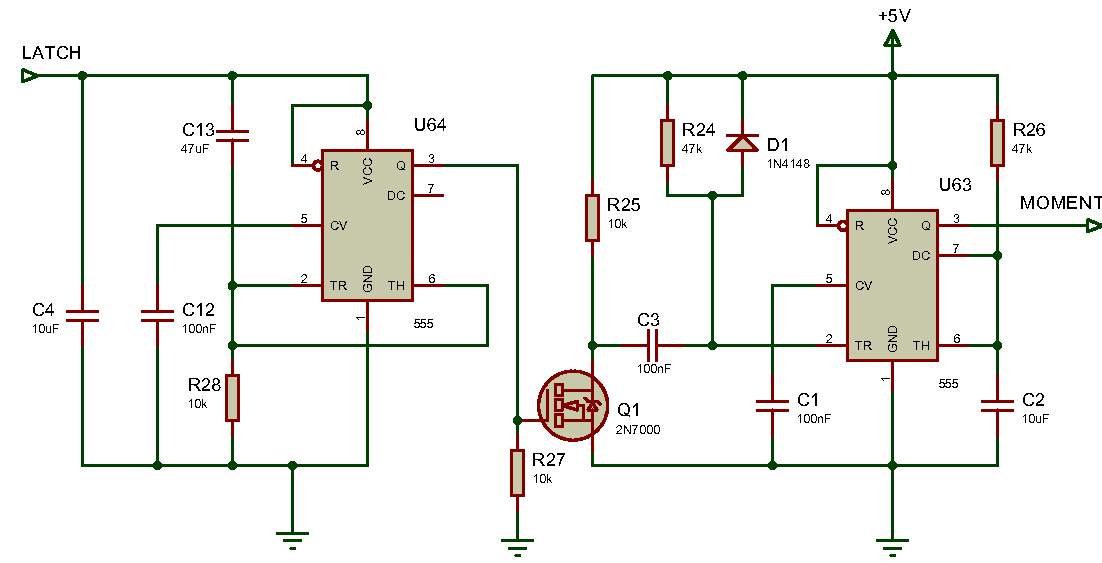
\includegraphics[scale = 0.7]{Graphics/DELAY/DELAY_PULSE.PDF}
    \caption{Delayed impulse after a PGT}
    \label{fig:DELAY_IMPULSE}
\end{figure}


When Q1 is off, that is, when the output of the first monostable is 0V, C3 is in short circuit, meaning that both its leads are at 5V due to the pull-ups R24 and R25, so the voltage drop across it is 0V. The voltage at the Trigger pin (Pin 2) is 5V as well, which means that the output Q (Pin 3) is off, as we need a voltage equal or lower than $V_{cc}/3$ at the Trigger pin to turn it on.\medskip

Once the N-Channel Mosfet is turned on by the first 555, the capacitor is grounded and an RC network is formed by R24 and C3. The voltage in the capacitor is 0V initially, so the voltage in the Trigger pin is 0V as well, turning the output on. As soon as C3 charges, The voltage at the trigger returns to 5V again and the output is switched off. In essence, this simulates the press of a button. \medskip

Q1 is an arbitrary N-Channel Mosfet and R27 is there to discharge its internal capacitor. \medskip

In our circuit, we have used this circuit three times to accomplish various duties such as:

\begin{itemize}
    \item Auto starting the system. (See \textbf{Subsubsection \ref{sec:AUTOSTART}})
    \item Resetting the system once the execution of the code is finished. (\textbf{See Subsection \ref{sec:GENERAL_RESET}})
    \item To wait a few ms before showing the Open/Error message during which the introduced number is shown. (\textbf{See Subsections \ref{sec:PASS_CHECK} and \ref{sec:OPEN_ERROR}})
\end{itemize}